\documentclass[a4paper,12pt,twoside]{memoir}

% Castellano
\usepackage[spanish,es-tabla]{babel}
\selectlanguage{spanish}
\usepackage[utf8]{inputenc}
\usepackage[T1]{fontenc}
\usepackage{lmodern} % Scalable font
\usepackage{microtype}
\usepackage{placeins}

\RequirePackage{booktabs}
\RequirePackage[table]{xcolor}
\RequirePackage{xtab}
\RequirePackage{multirow}

% Links
\usepackage[colorlinks]{hyperref}
\hypersetup{
	allcolors = {red}
}

% Ecuaciones
\usepackage{amsmath}

% Rutas de fichero / paquete
\newcommand{\ruta}[1]{{\sffamily #1}}

% Párrafos
\nonzeroparskip


% Imagenes
\usepackage{graphicx}
\newcommand{\imagen}[2]{
	\begin{figure}[!h]
		\centering
		\includegraphics[width=0.9\textwidth]{#1}
		\caption{#2}\label{fig:#1}
	\end{figure}
	\FloatBarrier
}

\newcommand{\imagenflotante}[2]{
	\begin{figure}%[!h]
		\centering
		\includegraphics[width=0.9\textwidth]{#1}
		\caption{#2}\label{fig:#1}
	\end{figure}
}



% El comando \figura nos permite insertar figuras comodamente, y utilizando
% siempre el mismo formato. Los parametros son:
% 1 -> Porcentaje del ancho de página que ocupará la figura (de 0 a 1)
% 2 --> Fichero de la imagen
% 3 --> Texto a pie de imagen
% 4 --> Etiqueta (label) para referencias
% 5 --> Opciones que queramos pasarle al \includegraphics
% 6 --> Opciones de posicionamiento a pasarle a \begin{figure}
\newcommand{\figuraConPosicion}[6]{%
  \setlength{\anchoFloat}{#1\textwidth}%
  \addtolength{\anchoFloat}{-4\fboxsep}%
  \setlength{\anchoFigura}{\anchoFloat}%
  \begin{figure}[#6]
    \begin{center}%
      \Ovalbox{%
        \begin{minipage}{\anchoFloat}%
          \begin{center}%
            \includegraphics[width=\anchoFigura,#5]{#2}%
            \caption{#3}%
            \label{#4}%
          \end{center}%
        \end{minipage}
      }%
    \end{center}%
  \end{figure}%
}

%
% Comando para incluir imágenes en formato apaisado (sin marco).
\newcommand{\figuraApaisadaSinMarco}[5]{%
  \begin{figure}%
    \begin{center}%
    \includegraphics[angle=90,height=#1\textheight,#5]{#2}%
    \caption{#3}%
    \label{#4}%
    \end{center}%
  \end{figure}%
}
% Para las tablas
\newcommand{\otoprule}{\midrule [\heavyrulewidth]}
%
% Nuevo comando para tablas pequeñas (menos de una página).
\newcommand{\tablaSmall}[5]{%
 \begin{table}
  \begin{center}
   \rowcolors {2}{gray!35}{}
   \begin{tabular}{#2}
    \toprule
    #4
    \otoprule
    #5
    \bottomrule
   \end{tabular}
   \caption{#1}
   \label{tabla:#3}
  \end{center}
 \end{table}
}

%
% Nuevo comando para tablas pequeñas (menos de una página).
\newcommand{\tablaSmallSinColores}[5]{%
 \begin{table}[H]
  \begin{center}
   \begin{tabular}{#2}
    \toprule
    #4
    \otoprule
    #5
    \bottomrule
   \end{tabular}
   \caption{#1}
   \label{tabla:#3}
  \end{center}
 \end{table}
}

\newcommand{\tablaApaisadaSmall}[5]{%
\begin{landscape}
  \begin{table}
   \begin{center}
    \rowcolors {2}{gray!35}{}
    \begin{tabular}{#2}
     \toprule
     #4
     \otoprule
     #5
     \bottomrule
    \end{tabular}
    \caption{#1}
    \label{tabla:#3}
   \end{center}
  \end{table}
\end{landscape}
}

%
% Nuevo comando para tablas grandes con cabecera y filas alternas coloreadas en gris.
\newcommand{\tabla}[6]{%
  \begin{center}
    \tablefirsthead{
      \toprule
      #5
      \otoprule
    }
    \tablehead{
      \multicolumn{#3}{l}{\small\sl continúa desde la página anterior}\\
      \toprule
      #5
      \otoprule
    }
    \tabletail{
      \hline
      \multicolumn{#3}{r}{\small\sl continúa en la página siguiente}\\
    }
    \tablelasttail{
      \hline
    }
    \bottomcaption{#1}
    \rowcolors {2}{gray!35}{}
    \begin{xtabular}{#2}
      #6
      \bottomrule
    \end{xtabular}
    \label{tabla:#4}
  \end{center}
}

%
% Nuevo comando para tablas grandes con cabecera.
\newcommand{\tablaSinColores}[6]{%
  \begin{center}
    \tablefirsthead{
      \toprule
      #5
      \otoprule
    }
    \tablehead{
      \multicolumn{#3}{l}{\small\sl continúa desde la página anterior}\\
      \toprule
      #5
      \otoprule
    }
    \tabletail{
      \hline
      \multicolumn{#3}{r}{\small\sl continúa en la página siguiente}\\
    }
    \tablelasttail{
      \hline
    }
    \bottomcaption{#1}
    \begin{xtabular}{#2}
      #6
      \bottomrule
    \end{xtabular}
    \label{tabla:#4}
  \end{center}
}

%
% Nuevo comando para tablas grandes sin cabecera.
\newcommand{\tablaSinCabecera}[5]{%
  \begin{center}
    \tablefirsthead{
      \toprule
    }
    \tablehead{
      \multicolumn{#3}{l}{\small\sl continúa desde la página anterior}\\
      \hline
    }
    \tabletail{
      \hline
      \multicolumn{#3}{r}{\small\sl continúa en la página siguiente}\\
    }
    \tablelasttail{
      \hline
    }
    \bottomcaption{#1}
  \begin{xtabular}{#2}
    #5
   \bottomrule
  \end{xtabular}
  \label{tabla:#4}
  \end{center}
}



\definecolor{cgoLight}{HTML}{EEEEEE}
\definecolor{cgoExtralight}{HTML}{FFFFFF}

%
% Nuevo comando para tablas grandes sin cabecera.
\newcommand{\tablaSinCabeceraConBandas}[5]{%
  \begin{center}
    \tablefirsthead{
      \toprule
    }
    \tablehead{
      \multicolumn{#3}{l}{\small\sl continúa desde la página anterior}\\
      \hline
    }
    \tabletail{
      \hline
      \multicolumn{#3}{r}{\small\sl continúa en la página siguiente}\\
    }
    \tablelasttail{
      \hline
    }
    \bottomcaption{#1}
    \rowcolors[]{1}{cgoExtralight}{cgoLight}

  \begin{xtabular}{#2}
    #5
   \bottomrule
  \end{xtabular}
  \label{tabla:#4}
  \end{center}
}


















\graphicspath{ {./img/} }

% Capítulos
\chapterstyle{bianchi}
\newcommand{\capitulo}[2]{
	\setcounter{chapter}{#1}
	\setcounter{section}{0}
	\chapter*{#2}
	\addcontentsline{toc}{chapter}{#2}
	\markboth{#2}{#2}
}

% Apéndices
\renewcommand{\appendixname}{Apéndice}
\renewcommand*\cftappendixname{\appendixname}

\newcommand{\apendice}[1]{
	%\renewcommand{\thechapter}{A}
	\chapter{#1}
}

\renewcommand*\cftappendixname{\appendixname\ }

% Formato de portada
\makeatletter
\usepackage{xcolor}
\newcommand{\tutor}[1]{\def\@tutor{#1}}
\newcommand{\course}[1]{\def\@course{#1}}
\definecolor{cpardoBox}{HTML}{E6E6FF}
\def\maketitle{
  \null
  \thispagestyle{empty}
  % Cabecera ----------------
\noindent
\includegraphics[width=\textwidth]{cabecera}\vspace{1cm}%
  \vfill
  % Título proyecto y escudo informática ----------------
  \colorbox{cpardoBox}{%
    \begin{minipage}{.8\textwidth}
      \vspace{.5cm}\Large
      \begin{center}
      \textbf{TFG del Grado en Ingeniería Informática}\vspace{.6cm}\\
      \textbf{\LARGE\@title{}}
      \end{center}
      \vspace{.2cm}
    \end{minipage}

  }%
  \hfill\begin{minipage}{.20\textwidth}
    
\includegraphics[width=\textwidth]{escudoInfor}
  \end{minipage}
  \vfill
  % Datos de alumno, curso y tutores ------------------
  \begin{center}%
  {%
    \noindent\LARGE
    Presentado por \@author{}\\ 
    en Universidad de Burgos --- \@date{}\\
    Tutor: \@tutor{}\\
  }%
  \end{center}%
  \null
  \cleardoublepage
  }
\makeatother

\newcommand{\nombre}{Francisco Saiz Güemes} %%% cambio de comando

% Datos de portada
\title{Weblectric 2018}
\author{\nombre}
\tutor{Álvar Arnaiz Gonzales - Jesús Maudes Raedo}
\date{\today}

\begin{document}

\maketitle


\newpage\null\thispagestyle{empty}\newpage


%%%%%%%%%%%%%%%%%%%%%%%%%%%%%%%%%%%%%%%%%%%%%%%%%%%%%%%%%%%%%%%%%%%%%%%%%%%%%%%%%%%%%%%%
\thispagestyle{empty}


\noindent
\includegraphics[width=\textwidth]{cabecera}\vspace{1cm}

\noindent D. nombre tutor, profesor del departamento de nombre departamento, área de nombre área.

\noindent Expone:

\noindent Que el alumno D. \nombre, con DNI 71567002H, ha realizado el Trabajo final de Grado en Ingeniería Informática titulado título de TFG. 

\noindent Y que dicho trabajo ha sido realizado por el alumno bajo la dirección del que suscribe, en virtud de lo cual se autoriza su presentación y defensa.

\begin{center} %\large
En Burgos, {\large \today}
\end{center}

\vfill\vfill\vfill

% Author and supervisor
\begin{minipage}{0.45\textwidth}
\begin{flushleft} %\large
Vº. Bº. del Tutor:\\[2cm]
D. nombre tutor
\end{flushleft}
\end{minipage}
\hfill
\begin{minipage}{0.45\textwidth}
\begin{flushleft} %\large
Vº. Bº. del co-tutor:\\[2cm]
D. nombre co-tutor
\end{flushleft}
\end{minipage}
\hfill

\vfill

% para casos con solo un tutor comentar lo anterior
% y descomentar lo siguiente
%Vº. Bº. del Tutor:\\[2cm]
%D. nombre tutor


\newpage\null\thispagestyle{empty}\newpage




\frontmatter

% Abstract en castellano
\renewcommand*\abstractname{Resumen}
\begin{abstract}
En este primer apartado se hace una \textbf{breve} presentación del tema que se aborda en el proyecto.
\end{abstract}

\renewcommand*\abstractname{Descriptores}
\begin{abstract}
Palabras separadas por comas que identifiquen el contenido del proyecto Ej: servidor web, buscador de vuelos, android \ldots
\end{abstract}

\clearpage

% Abstract en inglés
\renewcommand*\abstractname{Abstract}
\begin{abstract}
A \textbf{brief} presentation of the topic addressed in the project.
\end{abstract}

\renewcommand*\abstractname{Keywords}
\begin{abstract}
keywords separated by commas.
\end{abstract}

\clearpage

% Indices
\tableofcontents

\clearpage

\listoffigures

\clearpage

\listoftables
\clearpage

\mainmatter
\capitulo{1}{Introducción}

La optimización consiste en la selección del mejor elemento (con respecto a algún criterio) dentro de un conjunto de elementos. Si hablamos de problemas de optimización, el proceso consiste en minimizar o maximizar una función real escogiendo de manera sistemática valores de entrada (tomados de un conjunto permitido) y calculando el valor de la función~\cite{wiki:optimizacion}.

Existen diferentes métodos de optimización a los que se hará referencia en algún punto de la documentación, sin embargo, el proyecto está enfocado a la administración a través de una aplicación web de unos datos que nos facilita el investigador fruto de la ejecución de un algoritmo multi-objetivo llamado \textit{Nondominated Sorting Genetic Algorithm II (NSGA-II)}~\cite{pdf:nsga-ii}.

Para la administración de todos estos datos, en la figura~\ref{fig:weblectric}, presentamos \textit{Weblectric}, una aplicación desarrollada por petición del investigador residente en México, que desempeñará la función del cliente durante el desarrollo del proyecto. El objetivo es darle la posibilidad de administrar los datos y ejecutar su propio algoritmo desde la web.

A lo largo del proyecto podremos ver su estructura, el \textit{framework} utilizado, su diseño y algunas librerías de interés para leer y escribir datos con PHP en las hojas de cálculo. De la misma manera, reflejaremos los problemas detectados, cómo se han resuelto y qué lineas de futuro marcamos en el horizonte para continuar con el desarrollo de \textit{Weblectric}. 

\begin{figure}[ht]
	\centering
	
\includegraphics[width=0.4\textwidth]{/weblectric/logo}
	\caption{Weblectric.}
	\label{fig:weblectric}
\end{figure}
\capitulo{2}{Objetivos del proyecto}

Unificando y buscando complementar nuestros conocimientos y oportunidades con las necesidades manifestadas por el cliente, podríamos hablar de los siguientes objetivos:

\section{Objetivos generales}

Como objetivos técnicos propiamente del proyecto, podríamos destacar:

\begin{itemize}
	\item Conocer el funcionamiento general del algoritmo NSGA-II, u8n algoritmo de optimización.
	
	\item Dar soporte a través de una aplicación web a los resultados obtenidos mediante la ejecución del algoritmo de optimización.
	\begin{itemize}
		\item Una administración que permita crar, editar y eliminar cualquiera de las entidades.
		\item Una pantalla de simulación del algoritmo.
	\end{itemize}
	\item Aprender a emular en nuestra máquina, un servidor APACHE que nos permita desarrollar en nuestro entorno local.
	
	\item Familiarizarme con CakePHP. Un framework de desarrollo en Php con arquitectura MVC\footnote{MVC: Modelo Vista Controlador}.
	
	\item Conectar la aplicación con una base de datos MySql que nos permita manejar los datos proporcionados por el cliente.
	
	\item Alojar nuestros contenidos en un servidor al que accederemos mediante un cliente FTP\footnote{Nosotros utilizaremos Filezilla}.
\end{itemize}

\section{Objetivos personales}

Como objetivos quizá más personales que tambien me gustaría incluir para lograr alcanzar con el desarrollo de este proyecto, podríamos incluir:

\begin{itemize}
	\item Conocer mis tiempos y calcular costes de desarrolo con la idea de optimizar el rendimiento y planificación de mi tiempo.
	
	\item Aprender a adelantarme a las necesidades del cliente, aportándole una solución concreta, real y efectiva a sus necesidades.
	
	\item Viendo que las puertas al mundo profesional se me abren por este camino, me parece interesante complementar los conocimientos obtenidos durante estos años en la universidad con otros lenguajes de programación complementarios a PHP, los cuales utilizaré tambien en el desarrollo de la aplicación.
\end{itemize}

Como objetivo final del proyecto y visión de futuro para los próximos proyectos, me gustaría aprender a detectar las necesidades del cliente con la finalidad de generarle el máximo valor de negocio posible cubriendo todas sus necesidades.

\capitulo{3}{Conceptos teóricos}

Aunque el proyecto está enfocado a la administración a través de una aplicación web de unos datos que nos facilita el cliente, la base del proyecto se cimienta sobre un algoritmo de optimización capaz de proporcionarnos soluciones acerca de la mejor distribución de plantas energéticas en distintas regiones. 

Antes de explicar cómo se ha enfocado el planteamiento de la aplicación, es necesario hablar un poco sobre la optimización.

\section{Optimización}

\subsection{¿Qué es la optimización?}

Podríamos referirnos a la optimización como un proceso de selección del mejor elemento (con respecto a algún criterio) dentro de un conjunto de elementos disponibles~\cite{wiki:optimizacion}.

Si hablamos de problemas de optimización, el proceso consiste en minimizar o maximizar una función real escogiendo de manera sistemática valores de entrada (tomados de un conjunto permitido) y calculando el valor de la función~\cite{wiki:optimizacion}.

\subsection{Optimización clásica vs. Metaheurística}

La optimización clásica garantiza el óptimo numérico global y permite un numero elevado de restricciones. Algún método clásico es:
\begin{itemize}
	\item Programación lineal~\cite{web:programacionLineal}.
	\item Programación cuadrática~\cite{web:programacionCuadratica}.
	\item Programación no lineal~\cite{web:programacionNoLineal}.
	\item Programación dinámica~\cite{web:programacionDinamica}.
	\item Teoría de grafos u optimización en redes~\cite{pdf:teoriaGrafos}.
\end{itemize}

La optimización metaheurística trata de imitar fenómenos sencillos ocurrentes en la naturaleza, mecanismos específicos para evitar óptimos locales y tener una mirada mas "global". No garantizan la obtención de un óptimo absoluto así como tampoco permiten un gran número de restricciones.

Son soluciones aplicadas generalmente a problemas combinatorios que exploran un gran número de soluciones en un tiempo muy corto.

Algún método metaheurístico es:
\begin{itemize}
	\item Algoritmos evolutivos (genéticos)~\cite{pdf:algoritmosGeneticos}.
	\item Recocido o simulado~\cite{web:recocidoSimulado}.
	\item Sistemas multiagente~\cite{web:sistemasMultiagente}.
\end{itemize}

En esta aplicación, al igual que en muchas otras, se utilizan algoritmos de optimización metaherísticos porque el cálculo de un óptimo global es imposible de obtener en un tiempo razonable. Los métodos metaheurísticos, ofrecen un óptimo "razonablemente" bueno.

\subsection{Componentes}
A continuación, se van a describir los componentes de un sistema de optimización~\cite{pdf:optimizacion}.

\subsubsection{Función objetivo}
Medida cuantitativa de un sistema que se desea maximizar o minimizar.

\subsubsection{Variables}
Podemos hablar de ellas como las decisiones que afectan al valor de la función objetivo. Pueden ser dependientes o independientes.

\subsubsection{Restricciones}
Conjunto de relaciones que las variables están obligadas a satisfacer.

\subsubsection{Ejemplos básicos}

Por ejemplo: Un problema de optimización puede ser representado de la siguiente forma:

Dada: una función $f : A \rightarrow R$

Buscar: un elemento $x_{0}$ en $A$, tal que $f(x_{0}) \leq f(x)$ para todo $x$ en $A$ si hablamos de minimización, o $f(x_{0}) \geq f(x)$ para todo $x$ en $A$ si se trata de un problema de maximización.

En nuestro ejemplo, $A$ sería un subconjunto del \textit{espacio euclídeo}. Si trabajamos con una dimensión, denominaríamos \textit{espacio euclídeo} a una recta que va desde $-\infty$ hasta $+\infty$. En cambio, si trabajamos en dos dimensiones, el \textit{espacio euclídeo} sería un plano con infinitas rectas y puntos.
La función $f$ sería la función objetivo y se hace referencia a ella como función de costo en los problemas de 
minimización y función de utilidad en los problemas de maximización.

El objetivo de todos los problemas de optimización es encontrar el valor que deben tomar las variables para hacer óptima la función objetivo satisfaciendo el conjunto de restricciones. 

Sin embargo, cabe destacar que dentro de los problemas de optimización tenemos dos tipos:
\begin{itemize}
	\item Mono-objetivo.
	\item Multi-objetivo.
\end{itemize}

La diferencia entre ambos es que en los primeros solo hay un objetivo mientras que en los segundos hay más de uno y además pueden y suelen ir en direcciones opuestas.

Centrándonos de nuevo en nuestro análisis, la solución proporcionada para resolver el problema viene de parte de un algoritmo multi-objetivo llamado \textit{Nondominated Sorting Genetic Algorithm II (NSGA-II)}~\cite{pdf:nsga-ii}.

\section{NSGA-II}

Implementando esta solución, la meta a la que se quiere llegar es a encontrar un vector de variables $x=(x_1,x_2,…x_j)$ que cumpla con todas las restricciones y condiciones, donde las funciones objetivos resultantes sean optimizadas~\cite{pdf:algoritmo}.

Se denomina espacio de solución al conjunto de todas las combinaciones posibles. Es denotado mediante: $fn(x)=z=(z_1,z_2,…z_M)$. 

Sin embargo, en los problemas multiobjetivo, entran en juego simultáneamente funciones de minimizar y de maximizar.

Para llegar a una solución, en los problemas multiobjetivo, se introduce un nuevo operador, dominancia. Que define: una solución 
$x(1)$ predomina sobre otra solución $x(2)$ si se cumplen las siguientes condiciones~\cite{pdf:nsga-ii}:

\begin{itemize}
	\item La solución $x(1)$ no siempre es de menor calidad que $x(2)$ en todos los objetivos.
	\item Al menos en uno de los objetivos, la solución $x(1)$ es estrictamente mejor que $x(2)$.
\end{itemize}

Utilizando estas reglas de manera iterativa sobre un conjunto de soluciones de un problema de optimización multiobjetivo, se puede llegar a establecer cuáles son las alternativas dominantes. Las conocemos como \textit{Conjunto No Dominado}.
El resto de soluciones pasan a formar parte del \textit{Conjunto de Soluciones Dominadas}. 

Logrando establecer este conjunto de Soluciones Dominantes en un espacio objetivo, podemos hablar de \textit{Frente óptimo de Pareto}~\cite{img:frente_pareto}. (Figura~\ref{fig:frentePareto})

\begin{figure}[ht]
	\centering
	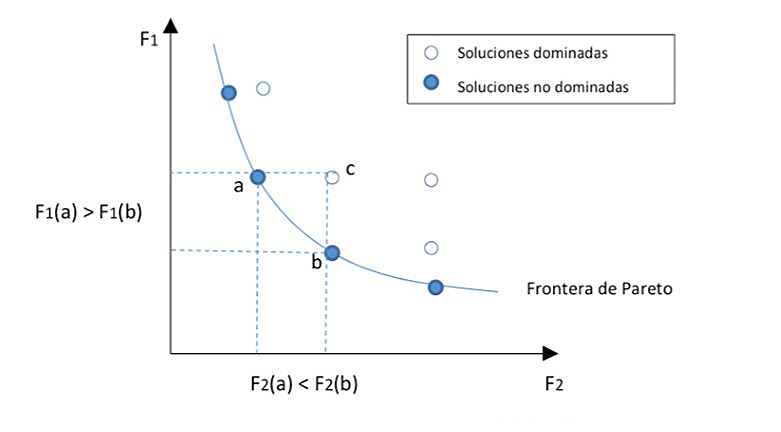
\includegraphics[width=1\textwidth]{/conceptosTeoricos/frentePareto}
	\caption{Frente de pareto en un problema de minimización. Ilustración extraida de~\cite{img:frente_pareto}.}
	\label{fig:frentePareto}
\end{figure}
\capitulo{4}{Técnicas y herramientas}

Para el desarrollo del proyecto y para lograr alcanzar tanto los objetivos académicos como personales propuestos anteriormente, he considerado de utilidad las siguientes técnicas y herramientas.

\section{Gestión del proyecto y control de versiones}

\subsection{Gestión del proyecto}

A la hora de gestionar un proyecto, podemos clasificar el método usado para su gestión en dos grandes grupos: metodología tradicional y metodología ágil.

Analizando las diferencias entre ellas podemos afirmar~\cite{web:diferencias-metodologias}:

\\texttt{begin}{itemize}
	\item En la metodología tradicional, esta presente la figura de un Project Manager que basa sus conocimientos en el \textit{Project Management Body of Knowledge}\footnote{PMBoK. Libro donde se recogen técnicas y acciones a llevar a cabo dentro de un proyecto para obtener un resultado próspero.}.
	\item La metodología tradicional se centra en un enfoque proactivo y predictivo. Busca desde los orígenes del proyecto definir todo lo definible antes de empezar, anticiparse a cualquier cambio, buscar proyección, es decir, dar un alcance lo más completo posible y ajustar el coste al máximo.
	
	\item La metodología ágil surge como necesidad del cliente a proyectos no muy grandes. No existe una necesidad por parte del cliente de una planificación inicial exhaustiva, sino que necesita un producto en un espacio corto de tiempo y no hay tiempo para grandes planificaciones.
	\item Es probable que el producto demandado por el cliente en un principio, sea diferente del demandado a final del proyecto. Esto se debe al continuo cambio sobretodo en el mundo de las TIC. El cliente sabe qué necesita pero desconoce cómo se va a concretar a $X$ días vista
\end{itemize}

Estando delante de un proyecto no muy grande y aprovechando los conocimientos recibidos en el grado, hemos decidido utilizar una metodología ágil para gestionar nuestro proyecto.

\subsubsection{SCRUM}

\textit{Scrum}\footnote{No son siglas. Su significado viene de la palabra melé. Jugada de rugby en la que jugadores de ambos equipos se agrupan en una formación en la cual lucharán por obtener el balón que se introduce por el centro. \cite{web:scrum_origen}}~\cite{web:scrum} es uno de los métodos ágiles más extendidos. Se trata de un método incremental e iterativo que divide el desarrollo del producto en ciclos llamados \textit{sprints}.

Al inicio de cada \textit{sprint}, se realiza una reunión entre todos los integrantes del proyecto donde se definen los objetivos y requisitos de cada ciclo. Cada una de esas tareas se denomina \textit{issues}.

Este tipo de metodología ha sido muy eficiente en el desarrollo. Una de las ventajas que nos ha proporcionado, ha sido la capacidad de reaccionar ante los cambios teniendo la oportunidad de ir creando en cada \textit{sprint}, especificaciones y requerimientos nuevos.

\subsubsection{ZenHub}

\textit{ZenHub} es una plataforma de gestión de proyectos que se integra en \textit{GitHub}, instalándose en el navegador mediante una extensión \footnote{Podemos descargarlo en \url{https://www.zenhub.com/}}.

Es una herramienta muy cómoda y visual, ya que permite administrar todos los elementos comentados anteriormente característicos de la metodología SCRUM. Destacar que ZenHub llama a los \textit{sprints}, \textit{milestones}. El resto de nomenclatura es igual.

En la figura \ref{fig:ZenHub} tenemos presentes las diferentes columnas del \textit{tablero}. Este elemento, es de gran utilidad para clasificar por \textit{milestones}, cada \textit{issue}.

\begin{figure}[ht]
	\centering
	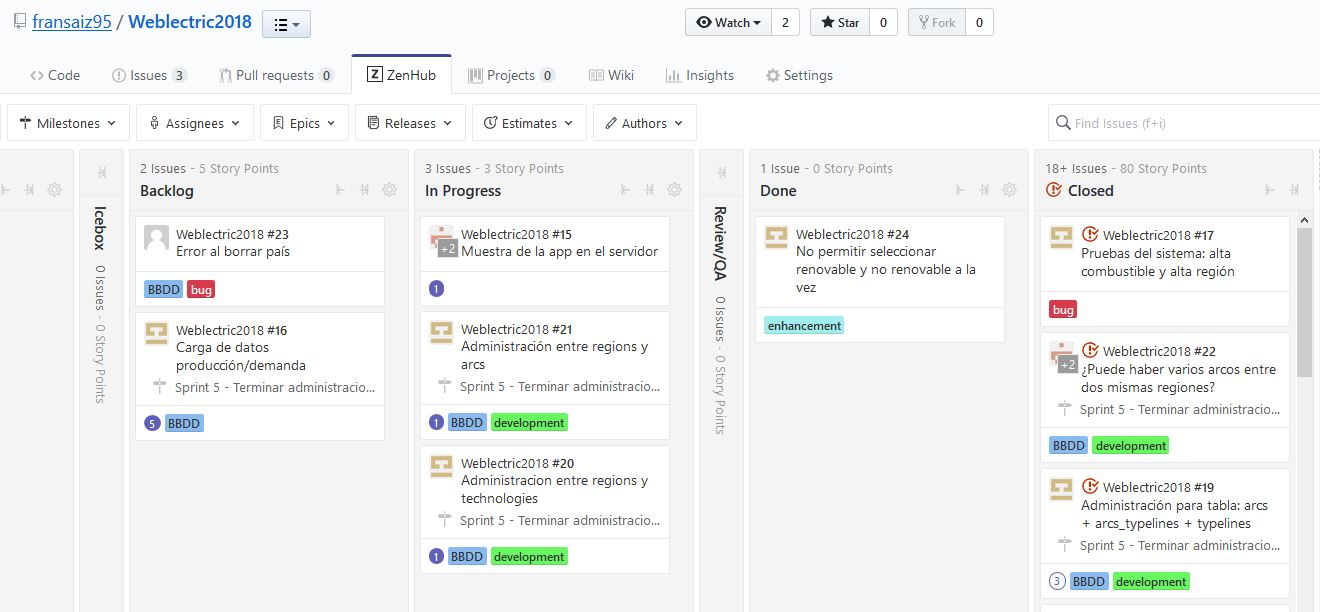
\includegraphics[width=1\textwidth]{/conceptosTeoricos/ZenHub}
	\caption{Ejemplo de nuestro tablero en \textit{ZenHub}.}
	\label{fig:ZenHub}
\end{figure}

\subsection{Control de versiones}

Como repositorio y control de versiones, hemos elegido \textit{Git} a través de la herramienta \textit{GitHub}\footnote{Software de código abierto y gratuito que permite un control de versiones a través de ramas (\textit{branchs}) en las que cada usuario puede editar y publicar cambios.}

GitHub es una plataforma online basada en Git, que permite la creación de repositorios tanto públicos como privados en los que posteriormente un equipo puede alojar su trabajo.

Además, GitHub ofrece una version para escritorio (\textit{GitHub Desktop}) con la que poder realizar subidas y bajadas (\textit{push - pull}) directamente desde el escritorio. Nosotros hemos utilizado \textit{Sourcetree}, un cliente Git que proporciona una interfaz amigable para interactuar con nuestros repositorios. Pertenece a la empresa \textit{Atlassian.}

A través del siguiente enlace, podemos acceder al proyecto \textit{Weblectric} que utiliza \textit{GitHub} como repositorio y control de versiones.

\url{https://github.com/fransaiz95/Weblectric2018}

\newpage

\section{Entorno de desarrollo}

Puesto que el objetivo principal del proyecto es construir una aplicación web dando soporte al cliente a que pueda cubrir sus necesidades, necesitamos un sitio donde alojar la aplicación. 

Antes de contratar ningún servicio externo, empezamos a desarrollar la aplicación en nuestro entorno local. Para ello necesitamos de la siguiente herramienta.

\subsection{XAMPP}

XAMPP es un paquete de software libre que consiste principalmente en el sistema de gestión de bases de datos \textit{MySQL}, el servidor web \textit{Apache} e intérpretes para lenguajes PHP y Perl~\cite{wiki:xampp}.

La ventaja de utilizar esta herramienta es que te ahorras el tiempo y la dificultad de configuración de cada uno de los servicios por separado. 

\subsection{HeidiSQL}

Aunque XAMPP trae consigo el servicio \textit{PhpMyAdmin} para gestionar las bases de datos \textit{MySQL}, nosotros hemos decidido utilizar \textit{HeidiSQL} ya que tiene una interfaz más amigable y permite más opciones.

\textit{HeidiSQL} es un software libre de código abierto que nos da la facilidad de conectarnos a servidores \textit{MySQL}.

Para administrar las bases de datos con esta herramienta, el usuario tiene que iniciar sesión en un servidor \textit{MySQL} local o remoto. 

\subsection{Filezilla}

Una vez que tenemos nuestro entorno de desarrollo en local, es común necesitar un servidor externo donde alojar tu aplicación. Para transferir los archivos al servidor, utilizamos \textit{Filezilla}. Un gestor \textit{FTP} de código abierto y software libre.

Tras establecer la conexión con el servidor, el manejo de los archivos y la navegación ente los directorios es fácil e intuitiva. Además, permite arrastrar y soltar, lo que facilita su uso.

\subsection{Visual Studio Code}

\textit{Visual Studio Code} es un editor de código fuente desarrollado por \textit{Microsoft}. Al incluir control integrado de \textit{Git}, hace que el resultado y el control de versiones de nuestro código sea más manejable.

No es un IDE como tal, pero gracias a numerosas extensiones hace que el trato con él sea mucho más satisfactorio. Acepta extensiones para hacer más fácil la lectura de los lenguajes \textit{PHP}, \textit{HTML}, \textit{CSS} y \textit{Javascript}. 



\subsection{Prepros}

\textit{Prepros} es una herramienta completa para desarrollo front-end\footnote{La parte del software que interactúa con los usuarios.}. Se trata de un compendio de funcionalidades que abarcan desde el desarrollo con lenguajes como CSS o Javascript, a la optimización de imágenes.

Además, en este trabajo, se utiliza como compilador de archivos \textit{*.scss} a \textit{*.css} pues el desarrollo se hace en \textit{Sass}, que es parecido a \textit{CSS}. Posteriormente se compila la estructura de archivos \textit{*.scss} en un \textit{*.css} general que utiliza la web.

Para una correcta estructuración de la hoja de estilos, en la figura \ref{fig:scss} podemos ver como se ha llevado a cabo.
Tenemos un directorio con cada uno de los archivos \textit{.scss} que se agrupan en un \textit{estilos.scss} que a su vez, siendo compilado con el \textit{Prepros}, genera un \textit{estilos.css}. Este archivo es de donde se nutre la aplicación web.

\begin{figure}[ht]
	\centering
	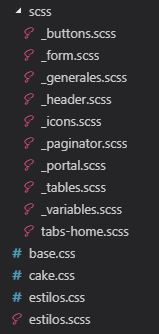
\includegraphics[width=0.3\textwidth]{/conceptosTeoricos/scss}
	\caption{Estructura de directorios de la hoja de estilos.}
	\label{fig:scss}
\end{figure}

\newpage

\section{Frameworks }

A continuación, iremos mencionando los diferentes \textit{frameworks (Entornos de trabajo)} que tras integrarlos entre sí, han hecho posible el desarrollo del proyecto.

\subsection{CakePHP}

\textit{CakePHP}~\cite{web:cakephp} es un \textit{framework} que facilita el desarrollo de aplicaciones web en PHP~\cite{wiki:cakephp}, utilizando el patrón de diseño MVC.

Facilita alguna ayuda para integrar \textit{Ajax}\footnote{Asynchronous JavaScript And XML (JavaScript asíncrono y XML), es una técnica de desarrollo web para crear aplicaciones interactivas~\cite{wiki:ajax}.}, Javascript, formularios... por lo que hace de su uso una herramienta interesante.

Además, vienen incluidos componentes de seguridad y de sesión que para una aplicación web siempre son interesantes.

En cuanto al Modelo Vista Controlador (figura~\ref{fig:mvc}), es un patrón de arquitectura de software que separa por una parte los datos y la lógica de una aplicación y por otra, la interfaz de usuario y el módulo encargado de gestionar los eventos y las comunicaciones. 

Separar las funciones de la aplicación en modelos, vistas y controladores hace que la aplicación sea mucho más ligera.

\begin{figure}[ht]
	\centering
	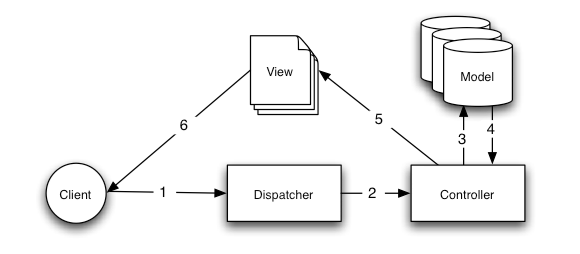
\includegraphics[width=0.9\textwidth]{/conceptosTeoricos/mvc}
	\caption{Ejemplo de arquitectura MVC. Ilustración extraida de~\cite{img:MVC}}
	\label{fig:mvc}
\end{figure}

\subsection{Zurb Foundation}

\textit{Foundation}~\cite{web:foundation} es un \textit{framework} de interfaz de usuario. Proporciona una cuadrícula responsive e incluye diferentes componentes:
\begin{itemize}
	\item Interfaz de usuario HTML y CSS.
	\item Plantillas.
	\item Fragmentos de código reutilizables.
	\item Tipografías.
	\item Formularios.
	\item Botones, barras de navegación y otros componentes de interfaz usuario.
	\item Extensiones de Javascript opcionales.
\end{itemize}

\textit{Foundation} está mantenida por \href{zurb.com}{Zurb} y es un proyecto de código abierto.

La competencia más directa de \textit{Foundation} como \textit{framework de CSS}, es \textit{Bootstrap}. Aunque en nuestra aplicación hemos usado \textit{Foundation}, cabe destacar que \textit{Bootstrap} ofrece unos servicios muy parecidos y una documentación de calidad como la de \textit{Foundation}. 

Por destacar alguna ventaja a favor de \textit{Bootstrap}, podemos decir que es más popular. Tiene más \textit{plugins} desarrollados y una comunidad de usuarios más grande, lo que facilita cualquier tipo de consulta en la web. Sin embargo, se ha decidido utilizar \textit{Foundation}, ya que viene con un archivo de ejemplo con el que hemos podido practicar y obtener conocimientos iniciales.

\capitulo{5}{Aspectos relevantes del desarrollo del proyecto}

\section{Tratamiento de datos}

\subsection{Lectura de datos}

Teniendo en cuenta los objetivos del proyecto ya comentados en apartados anteriores y queriendo lograr la construcción de una aplicación estable para que el usuario final pueda cargar sus datos y administrarlos, nos vimos obligados en primera instancia a buscar una librería en PHP capaz de leer una serie de datos de un Excel\footnote{El cliente nos envió así los datos que en un futuro desearía que fuesen administrables.} para posteriormente alojarlos en nuestra base de datos.

\subsubsection{Phpspreadsheet}

Para realizar esta operación conocíamos una librería llamada PHPExcel pero que actualmente a día de hoy está deprecada, por tanto, me vi en la obligación de investigar y buscar cuál era la solución actualmente. Así conseguimos dar con \textit{Phpoffice/Phpspreadsheet}. Mediante esta librería, que podemos encontrar su documentación en \href{https://phpspreadsheet.readthedocs.io/en/develop/}{phpspreadsheet}~\cite{web:spreadsheet}, podemos realizar lecturas y escrituras sobre un Excel. 

Como dejamos indicado en la figura~\ref{fig:spreadsheet} la librería cumple con creces nuestros requisitos además de ofrecernos alguna opción extra por si en un futuro o en próximas versiones del proyecto fuesen de interés~\cite{web:spreadsheet}.

\begin{figure}[ht]
	\centering
	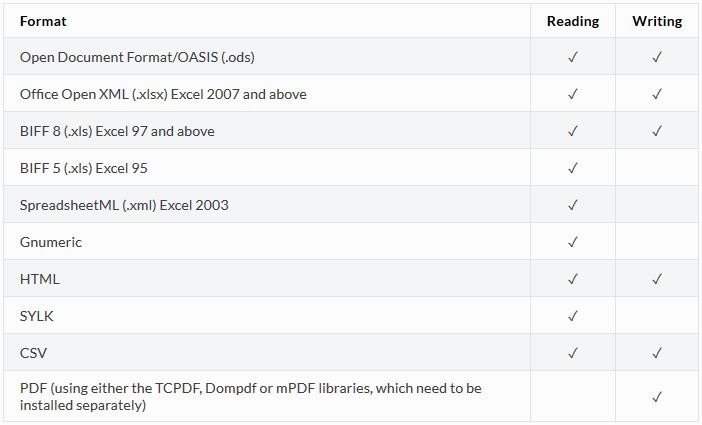
\includegraphics[width=0.9\textwidth]{/aspectosRelevantes/spreadsheet}
	\caption{Formatos de ficheros soportados por Spreadsheet.}
	\label{fig:spreadsheet}
\end{figure}

Para instalar librerías en CakePHP\footnote{Es el framework que hemos utilizadop para el desarrollo del proyecto}, hay diversas opciones, pero una de las más sencillas es utilizar \textit{Composer\footnote{Herramienta para la gestión de dependencias en PHP. Le permite declarar y administrar las bibliotecas de las que depende su proyecto.}}.

Para instalar \textit{Spreadsheet} en nuestro proyecto, nos dirigimos mediante comandos a la ruta de nuestro directorio que a tyravés de \textit{Composer} instalaremos la librería:

\begin{lstlisting}[language=bash]
composer require phpoffice/phpspreadsheet
\end{lstlisting}

Una vez la instalada, simplemente con la siguiente linea podemos importarlo en nuestro proyecto.

\begin{lstlisting}[language=PHP]
use PhpOffice\PhpSpreadsheet\Spreadsheet;
\end{lstlisting}

Como vemos, aunque el trato de los datos y la organización de los mismos si que ha sido un tema delicado, la instalación de las librerías en CakePHP es bastante sencillo.

\subsection{Escritura y almacenamiento de los datos}

En cuanto al manejo de los datos, aquí si que hemos tenido más problema. Se nos ha juntado la gran cantidad de datos con que el servidor donde hemos alojado esta primera versión de la aplicación no cuenta con recursos muy elevados.

Hemos tenido problemas a la hora de subir al servidor archivos muy grandes pues se agotaba la memoria al guardar los datos~\footnote{Rondando las 400K registros.} y se quedaba atascado. En nuestro entorno de desarrollo en local, el problema del tamaño de los archivos lo solucionamos modificando la propiedad $upload_max_filesize$ en el archivo $php.ini$ pero al no tener acceso a este archivo en el servidor, no podemos modificarlo. El problema de la memoria al guardar, no lo hemos podido solucionar aun utilizando la sentencia $ini_set('memory_limit', '-1');$ para indicar que puede utilizar toda la memoria que necesite y la sentencia $set_time_limit(0);$ para indicar que tiene el tiempo de ejecución ilimitado no lo hemos podido resolver en el entorno local pues se nos acababan los recursos.

Por esta razón es por lo que hemos tenido que fragmentar las cargas y administraciones de ciertos datos aunque lo ideal de cara a la usabilidad del usuario hubiera sido poder hacerlo todo en un mismo paso.

Para almacenar todos estos datos y poder dar al usuario la posibilidad de administrarlos, hemos construido una base de datos relacional. Para gestionarla, hemos utilizado el software \textit{HeidiSQL} que ofrece la posibilidad de conectarse a servidores \textit{MySQL}\footnote{Sistema de gestión de bases de datos relacional}.

\section{Estructura de la aplicación}

La estructura de directorios de nuestro proyecto lo podemos ver en la figura~\ref{fig:estructuraProyecto}. Destacamos los siguientes directorios:

\begin{itemize}
	\item \textit{config}: En la figura~\ref{fig:estructuraProyectoConfig} vemos los ficheros de configuración de nuestra aplicación. Con una importancia especial podemos destacar: 
	\begin{itemize}
		\item app.php: Archivo donde se establecen los parámetros de configuración para el email, la base de datos, los logs, la sesión, el debug, etc.
		\item constantes.php: Como indica el nombre del archivo, aquí se declaran clases con constantes comunes para poder usarlas desde el resto de la aplicación.
		\item paths.php: Definir variables globales para rutas de directorios concretos.
	\end{itemize}
		
	\item \textit{webroot}: Dentro de la estructura cliente-servidor, en la figura~\ref{fig:estructuraProyectoWebroot} encontramos lo relacionado con el cliente. Nuestra hoja de estilos, los archivos $*.js$, las imágenes, las fuentes y el favicon.pnp\footnote{Se conoce como favicon al icono que aparece en la pestaña del navegador junto con el nombre de la aplicación.}.
	
	\item \textit{src}: Aquí se almacenarán los archivos de tu aplicación.
\end{itemize}

\begin{figure}[ht]
	\centering
	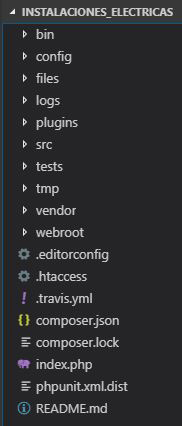
\includegraphics[width=0.3\textwidth]{/aspectosRelevantes/estructuraProyecto}
	\caption{Estructura general de un proyecto desarrollado con CakePHP.}
	\label{fig:estructuraProyecto}
\end{figure}

\begin{figure}[ht]
	\centering
	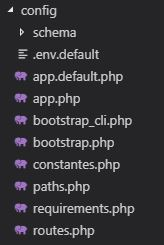
\includegraphics[width=0.3\textwidth]{/aspectosRelevantes/estructuraProyectoConfig}
	\caption{Directorio \textit{config} de nuestro proyecto.}
	\label{fig:estructuraProyectoConfig}
\end{figure}

\begin{figure}[ht]
	\centering
	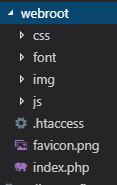
\includegraphics[width=0.2\textwidth]{/aspectosRelevantes/estructuraProyectoWebroot}
	\caption{Directorio \textit{webroot} de nuestro proyecto.}
	\label{fig:estructuraProyectoWebroot}
\end{figure}

No obstante, en la documentación oficial de \textit{CakePHP}~\cite{web:estructuraCarpetasCakePHP} se explican con mayor detalle cada uno de los directorios del proyecto.

\subsection{MVC}

El utilizar \textit{CakePHP} como \textit{framework} nos ha facilitado mucho la estructura del proyecto pues trabaja con el patrón MVC. De esta manera, como podemos ver en la figura \ref{fig:estructuraProyectoSrc}, tenemos bien separadas las tres partes fundamentales de la aplicación. 

\begin{figure}[ht]
	\centering
	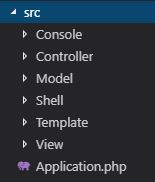
\includegraphics[width=0.2\textwidth]{/aspectosRelevantes/estructuraProyectoSrc}
	\caption{Directorio \textit{src} de nuestro proyecto.}
	\label{fig:estructuraProyectoSrc}
\end{figure}

Por un lado tenemos la conexión con nuestra base de datos en lo que serían los Modelos\footnote{Directorio \textit{Models}.}. Allí están la mayoría de consultas y operaciones contra la base de datos. 

Por otro lado tenemos la parte de los controladores\footnote{Directorio \textit{Controller}.}. que hacen de intermediarios entre la base de datos y la vista. Aquí albergamos la parte lógica de nuestra aplicación.

Por último las vistas\footnote{Directorio \textit{Templates}.}. Esto es lo que ve el usuario. Como ya hemos comentado, para facilitarnos el trabajo y aprovechar herramientas muy útiles ya creadas y puestas en el mercado, hemos utilizado \textit{Foundation 6.4.2}

Su implementación dentro del proyecto es muy sencilla, simplemente tenemos que colocar la siguiente linea en el \textit{layout\footnote{Vista definida como plantilla común al resto de vistas.}}:

\begin{lstlisting}[language=php]
echo $this->Html->css('lib/foundation-6.4.2/css/foundation.css');
\end{lstlisting}
\capitulo{6}{Trabajos relacionados}

En este apartado vamos a ir presentando algunos de los recursos competidores existentes en el mercado. Actualmente, ya hay varias plataformas que ofrecen un software personalizado para la optimización de energía y redes eléctricas. Iremos desglosando las diferentes opciones y destacando los detalles más relevantes.

\section{Energy Exemplar®}

\textit{Energy Exemplar®} presume de ser el líder del mercado en tecnología de simulación de energía basada en la optimización. 

Su paquete de software\footnote{Publican su primera versión en el año 2000.}, encabezado por \textit{Plexos} y \textit{Aurora}, se utiliza en todas las regiones del mundo para una amplia gama de aplicaciones, desde análisis a corto plazo hasta estudios de planificación a largo plazo. Permiten minimizar los costos operativos y de inversión, maximizar las ganancias y obtener pronósticos mucho mas precisos. Ofrecen sus servicios como el mejor software de simulación de energía eléctrica, gas y agua.  

La empresa se distribuye por todo el mundo contando con 9 oficinas repartidas por los cinco continentes.

\subsection{Plexos}

Como comentábamos antes, \textit{Plexos} es uno de los software que proporciona Energy Exemplar como solución~\cite{web:EnergyExemplarPlexos}. Combina técnicas de optimización basadas en matemática para el pronóstico con una experiencia gráfica de usuario muy potente y flexible. Presume de ofrecer lo último en gestión de datos orientados a objetos

\textit{Plexos Connect} mejora el software anterior al ofrecer computación distribuida\footnote{La computación distribuida es un modelo para resolver problemas de computación masiva utilizando un gran número de ordenadores organizados en clústeres.~\cite{web:computacionDistribuida}} a través de recursos locales y en la nube. Además ofrece ejecuciones por lotes completamente automatizadas y operaciones en tiempo real. Aloja los resultados de simulación en un repositorio central.

\subsection{Aurora}

Como afirman sus creadores~\cite{web:EnergyExemplarAurora}, \textit{Aurora} es un software de análisis y pronóstico de modelado eléctrico confiable, fácil de aprender y centrado en el usuario.

Los cambios rápidamente personalizables, sus bases de datos integradas y la interfaz fácil de usar proporcionan resultados muy satifactorios en el tiempo. Aurora permite el nivel más alto de integración de software, control de modelos y facilidad de intercambio de datos, ahorrando al usuario tiempo y dinero.

\section{Bentley Systems}

\textit{Bentley Systems} es una empresa de desarrollo de software que respalda las necesidades profesionales de los responsables de la creación y gestión de la infraestructura mundial: carreteras, aeropuertos, puentes, plantas industriales, eléctricas, etc.

Ofrece soluciones para todo el ciclo de vida del activo de infraestructura, adaptadas a las necesidades de las distintas profesiones que trabajarán con ese activo durante su ciclo de vida~\cite{web:bentleySystems}.

En la actualidad, la empresa tiene sede en: Estados Unidos, Irlanda y China.
\subsection{Advancement Academy}

Innovador programa que ofrece la posibilidad de coordinar equipos de ejecución complejos de arquitectura, ingeniería y construccion (AEC). Permite gestionar la complejidad de datos que se producen al incorporar a los contratistas.

Garantiza que sus colaboradores entiendan los procesos y productos a entregar que se esperan para una ejecución eficaz del proyecto. La herramienta ofrecerá un currículo específico para el proyecto que será escalable y flexible para adaptarse a cualquier situación~\cite{web:bentleySystemsAdvancementAcademies}.

Sus soluciones abarcan todo el ciclo de vida activo, desde el diseño hasta la construcción, pasando por la optimización de las centrales.

En el siguiente \href{https://www.bentley.com/es/project-profiles}{\textit{enlace}}, puede conocer algunos de los proyectos llevados a cabo por \textit{Bentley Systems}.

\section{LEAP}

\textit{LEAP}, el sistema de planificación de alternativas energéticas a largo plazo, es una herramienta de software adoptada y utilizada por 190 países en todo el mundo para el análisis de políticas energéticas y la evaluación del ahorro energético desarrollada en el Instituto de Medio Ambiente de Estocolmo~\cite{web:LEAP}.

Entre sus usuarios, tenemos presentes a académicos, agencias gubernamentales, organizaciones no gubernamentales, empresas consultoras y empresas de energía. Su uso varía desde ciudades y estados hasta aplicaciones nacionales, regionales y globales.

En los últimos tiempos, se está convirtiendo en el estándar de facto para los países que realizan una planificación integrada de recursos, evaluaciones de mitigación de gases de efecto invernadero (GEI) y Estrategias de Desarrollo de Baja Emisión (LEDS).

Al menos 32 países utilizaron el \textit{LEAP} para crear escenarios de energía y emisiones.

Es una herramienta de modelado integrada y basada en escenarios cuyo uso puede ser rastrear la producción, el consumo de energía y la extracción de recursos en todos los campos de una economía. 

De cara al usuario, cuenta con buena reputación porque ha sido capaz de hacer transparente el uso de conceptos complejos de análisis de energía. Del mismo modo, es flexible para usuarios que si cuentan con conocimientos a fondo y experiencia.

No es un modelo de un sistema de energía en particular. Es una herramienta que se puede utilizar para cubrir unas necesidades al crear modelos de diferentes sistemas de energía, donde cada modelo requiere estructuras de datos personales y únicas. Es compatible con una amplia gama de diferentes metodologías de modelado a medio y largo plazo~\cite{web:LEAP}.

Una gran parte de los estudios realizados, utilizan un período de pronóstico de entre 20 y 50 años. Sin embargo, aunque suele ser lo habitual, no siempre es así. Por ejemplo, para los cálculos del sector eléctrico, el año se suele dividir en diferentes ``intervalos de tiempo'' definidos por el usuario para representar periodos de tiempo como pueden ser temporadas, días o incluso horas con un valor especial en el día.

La aplicación se distribuye en diferentes vistas/pantallas que hace que el usuario pueda interaccionar con el software.

\begin{itemize}
	\item Vista de análisis.
	\item Herramientas para crear modelos.
	\item Informe de resultados.
	\item Balances de energía.
	\item Diagramas de Sankey.\footnote{Se utilizan para visualizar los flujos de balance de energía para cualquier área que se esté modelando en LEAP.}
	\item Base de datos de tecnología y medio ambiente (TED).
	\item Notas y documentación.
\end{itemize}

\section{OSeMOSYS}

Alternativa de código abierto para la evaluación integrada y la planificación energética a largo plazo. El proyecto nace en 2008 durante una presentación en París.

Diseñado para aquellos que no pueden o deseen hacer una inversión financiera inicial. Cuenta con una curva de aprendizaje rápida y un compromiso de operación de poco tiempo. Gracias a su transparencia, su uso se puede encontrar como herramienta de difusión y captación.

\textit{Model Management Infrastructure (MoManI)} es una interfaz de código abierto basada en navegador enfocada en el modelado de sistemas energéticos. La estructura de la aplicación ayuda a disminuir la complejidad perceptible de \textit{OSeMOSYS} y su estructura permite que varios equipos colabores simultáneamente desde cualquier parte del mundo.
El usuario puede actualizar y editar sin dificultad cualquier parte del proceso de modelado: desde la visualización de los resultados hasta las ecuaciones matemáticas subyacentes de \textit{OSeMOSYS}.

\section{Artículos científicos}

El 15 de Junio de 2016, Khizir Mahmud,Graham E. Town publicó un artículo~\cite{pdf:articuloAplicacionesRelacionadas} en el que hacía una revisión de las herramientas informáticas presentes en el mercado que sirviesen para modelar los requisitos energéticos de los vehículos eléctricos y su imparto en las redes de distribución de la energía. El artículo tuvo un gran impacto y los proyectos comentados anteriormente hacen referencia al artículo citado. 



\capitulo{7}{Conclusiones y Líneas de trabajo futuras}

En este capítulo se exponen las conclusiones obtenidas así como comentarios de interés útiles para poder seguir con el desarrollo del proyecto.

\section{Conclusiones}

Una vez finalizado el desarrollo y aun habiendo tenido problemas a la hora de comunicarse con el cliente, se han cumplido los requisitos y se ha obtenido un resultado satisfactorio que genera valor de negocio a las condiciones actuales en las que se encuentra el cliente, por tanto, podría afirmar que se han cumplido los objetivos.

A nivel personal, se han ampliado conocimientos con el uso de \textit{CakePHP} en su versión 3.5, pues siendo cierto que ya se había trabajado con este \textit{framework}, se había hecho con una versión antigua por lo que ha sido una buena oportunidad para reciclarse y ponerse al día. Unido a lo que sería el \textit{back-end}, también ha sido satisfactorio poder trabajar conjuntamente en el \textit{front-end} de la aplicación, pues el alumno no estaba acostumbrado a esas tareas.

Otro aspecto novedoso para el usuario que ha servido para ampliar conocimientos, ha sido el despliegue de la aplicación web en el servidor. Hasta ahora, aunque se había trabajado en proyectos ya desplegados, nunca había sido protagonista de la acción.

También, ha sido una buena oportunidad para refrescar conocimientos de bases de datos y volver a modelar diagramas entidad-relación y relacionales llevando a cabo a continuación el mapeo a sus correspondientes tablas. 

El trabajo con \textit{Scrum} como metodología ágil para gestionar el proyecto, ha sido muy útil y de gran ayuda, pues al tener que reestructurar la aplicación varias veces a petición del cliente, se ha sido capaz de adaptar los plazos y planificar cada uno de los \textit{sprints}. 

Para futuros proyectos, se va a adoptar la idea de poder trabajar con una base de datos de respaldo como se ha hecho aquí, pues ha sido muy útil para el usuario poder restablecer la base de datos a su versión de test mediante un botón. Gracias a esta funcionalidad, tanto el alumno como los tutores han podido probar la aplicación sin temor a dejar la base de datos en un estado inconsistente o que dificultara pruebas posteriores. Además, ha permitido detectar \textit{bugs} a lo largo del desarrollo y no únicamente en la parte final del proyecto.

\section{Líneas de trabajo futuras}

Para un desarrollo futuro, y a expensas de las necesidades del cliente y lo que se quiera implicar, podríamos enumerar una serie de mejoras que harían de la aplicación actual, un producto más robusto y mejor estructurado:

\begin{itemize}
	
	\item Replantear con el cliente si la estructura actual de la aplicación, diseñada a petición del cliente, es la más intuitiva y usable, pues por parte del alumno y tutores, se considera que puede haber otra estructuración mejor agrupada.
	
	\item Internacionalización de la aplicación para que pueda estar abierta a usuarios que no tengan por qué saber inglés.
	
	\item Valorar si merece la pena definir la topología de la red a través de mapas. A priori parece un trabajo bastante complejo, a falta de investigar la existencia de librerías que pudiesen ser de ayuda. Para representar los arcos entre dos regiones, se podría integrar en \textit{CakePHP} la librería de \textit{Google Maps} para hacer ese módulo más vistoso e intuitivo.
	
	\item Integrar en la aplicación en lugar de una base de datos \textit{MySQL}, una base de datos basada en grafos, como puede ser \textit{Neo4J}. Esta estructura es más apropiada para representar arcos y hacer consultas sobre ellos, pero se tendría que adaptar el código del algoritmo de optimización para que tomara los datos de estas nuevas consultas que en principio, tendrían mejores tiempos de respuesta. A su vez, este cambio conlleva que el algoritmo de optimización acceda al servidor de bases de datos, por lo que lo normal es que el algoritmo se ejecutase en el servidor.
	
	\item Para realizar pruebas sobre la aplicación, podría ser útil el uso de \textit{Selenium} como entorno de pruebas.
	
	\item En la actualidad, la aplicación no es \textit{responsive}, por lo que no es usable en versiones móviles. De cara a un desarrollo posterior, una vez que el algoritmo este preparado para ejecutarse desde el servidor, esta mejora aportaría bastante valor a la aplicación.
	
	\item Conseguir que el algoritmo de optimización se ejecute desde la web para mostrar los los resultados obtenidos en la propia aplicación.
	
\end{itemize}





\bibliographystyle{plain}
\bibliography{bibliografia}

\end{document}
